% Options for packages loaded elsewhere
\PassOptionsToPackage{unicode}{hyperref}
\PassOptionsToPackage{hyphens}{url}
\PassOptionsToPackage{dvipsnames,svgnames,x11names}{xcolor}
%
\documentclass[
  oneside]{book}
\usepackage{amsmath,amssymb}
\usepackage{lmodern}
\usepackage{iftex}
\ifPDFTeX
  \usepackage[T1]{fontenc}
  \usepackage[utf8]{inputenc}
  \usepackage{textcomp} % provide euro and other symbols
\else % if luatex or xetex
  \usepackage{unicode-math}
  \defaultfontfeatures{Scale=MatchLowercase}
  \defaultfontfeatures[\rmfamily]{Ligatures=TeX,Scale=1}
\fi
% Use upquote if available, for straight quotes in verbatim environments
\IfFileExists{upquote.sty}{\usepackage{upquote}}{}
\IfFileExists{microtype.sty}{% use microtype if available
  \usepackage[]{microtype}
  \UseMicrotypeSet[protrusion]{basicmath} % disable protrusion for tt fonts
}{}
\makeatletter
\@ifundefined{KOMAClassName}{% if non-KOMA class
  \IfFileExists{parskip.sty}{%
    \usepackage{parskip}
  }{% else
    \setlength{\parindent}{0pt}
    \setlength{\parskip}{6pt plus 2pt minus 1pt}}
}{% if KOMA class
  \KOMAoptions{parskip=half}}
\makeatother
\usepackage{xcolor}
\usepackage[margin=1in]{geometry}
\usepackage{longtable,booktabs,array}
\usepackage{calc} % for calculating minipage widths
% Correct order of tables after \paragraph or \subparagraph
\usepackage{etoolbox}
\makeatletter
\patchcmd\longtable{\par}{\if@noskipsec\mbox{}\fi\par}{}{}
\makeatother
% Allow footnotes in longtable head/foot
\IfFileExists{footnotehyper.sty}{\usepackage{footnotehyper}}{\usepackage{footnote}}
\makesavenoteenv{longtable}
\usepackage{graphicx}
\makeatletter
\def\maxwidth{\ifdim\Gin@nat@width>\linewidth\linewidth\else\Gin@nat@width\fi}
\def\maxheight{\ifdim\Gin@nat@height>\textheight\textheight\else\Gin@nat@height\fi}
\makeatother
% Scale images if necessary, so that they will not overflow the page
% margins by default, and it is still possible to overwrite the defaults
% using explicit options in \includegraphics[width, height, ...]{}
\setkeys{Gin}{width=\maxwidth,height=\maxheight,keepaspectratio}
% Set default figure placement to htbp
\makeatletter
\def\fps@figure{htbp}
\makeatother
\setlength{\emergencystretch}{3em} % prevent overfull lines
\providecommand{\tightlist}{%
  \setlength{\itemsep}{0pt}\setlength{\parskip}{0pt}}
\setcounter{secnumdepth}{5}
\newlength{\cslhangindent}
\setlength{\cslhangindent}{1.5em}
\newlength{\csllabelwidth}
\setlength{\csllabelwidth}{3em}
\newlength{\cslentryspacingunit} % times entry-spacing
\setlength{\cslentryspacingunit}{\parskip}
\newenvironment{CSLReferences}[2] % #1 hanging-ident, #2 entry spacing
 {% don't indent paragraphs
  \setlength{\parindent}{0pt}
  % turn on hanging indent if param 1 is 1
  \ifodd #1
  \let\oldpar\par
  \def\par{\hangindent=\cslhangindent\oldpar}
  \fi
  % set entry spacing
  \setlength{\parskip}{#2\cslentryspacingunit}
 }%
 {}
\usepackage{calc}
\newcommand{\CSLBlock}[1]{#1\hfill\break}
\newcommand{\CSLLeftMargin}[1]{\parbox[t]{\csllabelwidth}{#1}}
\newcommand{\CSLRightInline}[1]{\parbox[t]{\linewidth - \csllabelwidth}{#1}\break}
\newcommand{\CSLIndent}[1]{\hspace{\cslhangindent}#1}
\usepackage{booktabs}

\usepackage{tcolorbox}
\usepackage[T1]{fontenc}

\definecolor{dangcol}{RGB}{152,62,130}
\definecolor{warncol}{RGB}{245,220,112}
\definecolor{infocol}{RGB}{70,122,172}
\definecolor{trycol}{RGB}{97,88,156}

\newtcolorbox{dangerous}{
  colback=dangcol!10,
  colframe=dangcol,
  coltext=black,
  boxsep=5pt,
  arc=4pt
}

\newtcolorbox{warning}{
  colback=warncol!10,
  colframe=warncol,
  coltext=black,
  boxsep=5pt,
  arc=4pt
}

\newtcolorbox{info}{
  colback=infocol!10,
  colframe=infocol,
  coltext=black,
  boxsep=5pt,
  arc=4pt
}

\newtcolorbox{try}{
  colback=trycol!10,
  colframe=trycol,
  coltext=black,
  boxsep=5pt,
  arc=4pt
}
\ifLuaTeX
  \usepackage{selnolig}  % disable illegal ligatures
\fi
\usepackage[]{natbib}
\bibliographystyle{plainnat}
\IfFileExists{bookmark.sty}{\usepackage{bookmark}}{\usepackage{hyperref}}
\IfFileExists{xurl.sty}{\usepackage{xurl}}{} % add URL line breaks if available
\urlstyle{same} % disable monospaced font for URLs
\hypersetup{
  pdftitle={APA Open Guide},
  pdfauthor={OSM},
  colorlinks=true,
  linkcolor={Maroon},
  filecolor={Maroon},
  citecolor={Blue},
  urlcolor={blue},
  pdfcreator={LaTeX via pandoc}}

\title{APA Open Guide}
\author{OSM}
\date{2022-10-17}

\begin{document}
\maketitle

{
\hypersetup{linkcolor=}
\setcounter{tocdepth}{1}
\tableofcontents
}
\hypertarget{overview}{%
\chapter*{Overview}\label{overview}}
\addcontentsline{toc}{chapter}{Overview}

This guide is for editors, reviewers, and authors of APA submissions, to help them understand APA initiatives for open and transparent research, such as the TOP guidelines. The guiding principle is improving scientific rigour and increasing the transparency and accessibility of research; adjust any of the guidance for specific topics or circumstances in the service of those goals.

\textbf{The guide is in draft form. We are starting with guidance for editors and will be adding guidance for reviewers and authors soon. We welcome feedback and suggestions for further guidance.}

\hypertarget{top-guidelines}{%
\section{TOP Guidelines}\label{top-guidelines}}

\begin{itemize}
\tightlist
\item
  \href{https://www.apa.org/pubs/journals/resources/transparency-openness-promotion}{APA Transparency and Openness Promotion}
\item
  \href{https://www.cos.io/initiatives/top-guidelines}{COS TOP Guidelines}
\item
  \href{https://osf.io/9f6gx/}{OSF TOP Resources}
\end{itemize}

\hypertarget{getting-started-with-open-science}{%
\section{Getting Started with Open Science}\label{getting-started-with-open-science}}

\begin{itemize}
\item
  \href{https://psyarxiv.com/wu6sn}{An open science workflow for more credible, rigorous research} \citep{corker2021open}
\item
  \href{https://doi.org/10.1027/2151-2604/a000387}{Seven easy steps to open science} \citep{cruwell2019seven}
\item
  \href{https://doi.org/10.1525/collabra.18684}{Easing into open science: A guide for graduate students and their advisors} \citep{kathawalla2021easing}
\item
  \href{https://doi.org/10.1038/s41562-021-01269-4}{A community-sourced glossary of open scholarship terms} \citep{parsons2022community}
\item
  Spellman, B. A., Gilbert, E. A., \& Corker, K. S. (2018). Open science. In E. J. Wagenmakers (Volume Ed.) \& J. T. Wixted (Series Ed.) Stevens' Handbook of Experimental Psychology and Cognitive Neuroscience Volume 5: Methodology (4th ed.). Preprint at \url{https://osf.io/gv6r4/}
\end{itemize}

\hypertarget{part-editors}{%
\part{Editors}\label{part-editors}}

\hypertarget{editors-top}{%
\chapter{Transparency and Openness Statements}\label{editors-top}}

To enable readers to quickly and easily find open science disclosures, APA is requiring that authors include a subsection in their paper's Method section titled ``Transparency and Openness''. In this brief section, authors should disclose relevant details about seven TOP domains: availability of data, availability of code, availability of materials, citation to secondary data/code/materials (including citations of statistical software and packages), reporting standards, preregistration of study designs, and preregistration of analysis plans. The requirements for the information disclosed will depend on whether a journal has endorsed TOP level 1 or level 2.

\hypertarget{example-top-statement}{%
\section{Example TOP Statement}\label{example-top-statement}}

We report how we determined our sample size, all data exclusions, all manipulations, and all measures in the study, and we follow JARS \citep{kazak2018journal}. All data, analysis code, and research materials are available at {[}stable link to repository{]}. Data were analyzed using R, version 4.0.0 \citep{R} and the package lme4, version 1.1-27.1 \citep{lme4}. This study's design and its analysis were not pre-registered.

\hypertarget{resources}{%
\section{Resources}\label{resources}}

\begin{itemize}
\tightlist
\item
  \href{https://www.dropbox.com/s/8jv2n0j3mlkhkrj/TOP_GuidanceforReviewers.docx}{What to check} in transparency and openness statements for journals with TOP Level 1 or Level 2
\item
  \href{https://www.dropbox.com/s/rx616egpte53o9m/TOP_at_APA_withScript.pdf}{Introduction to TOP at APA for editors}
\item
  \href{https://www.apa.org/pubs/journals/resources/transparency-openness-promotion}{APA TOP}
\item
  \href{https://osf.io/9f6gx/}{OSF TOP}
\item
  \href{https://www.cos.io/initiatives/top-guidelines}{COS TOP}
\item
  \href{https://docs.google.com/document/d/10cMB2IT406gPAgCAORa5_UVI6Plrwvl4XjTsd0Ya_4s/edit}{TOP Mixed Level Journals}
\item
  \href{https://apastyle.apa.org/jars}{APA Journal Reporting Standards}
\end{itemize}

\hypertarget{editors-registered-reports}{%
\chapter{Registered Reports}\label{editors-registered-reports}}

From \href{https://www.cos.io/initiatives/registered-reports}{Center for Open Science}:

\begin{quote}
Registered Reports is a publishing format that emphasizes the importance of the research question and the quality of methodology by conducting peer review prior to data collection. High quality protocols are then provisionally accepted for publication if the authors follow through with the registered methodology.
\end{quote}

\begin{quote}
This format is designed to reward best practices in adhering to the hypothetico-deductive model of the scientific method. It eliminates a variety of questionable research practices, including low statistical power, selective reporting of results, and publication bias, while allowing complete flexibility to report serendipitous findings.
\end{quote}

Although not all APA journals offer the registered reports format, they may receive submissions that have been through the registered reports process at \href{https://rr.peercommunityin.org/}{PCI Registered Reports}, which will make all reviews and editorial communication publicly available. Such submissions can be treated like papers with a \protect\hyperlink{preregistration}{preregistration} (that has additionally been through a rigorous open review process).

\hypertarget{resources-1}{%
\section{Resources}\label{resources-1}}

\begin{itemize}
\tightlist
\item
  \href{https://osf.io/rr/}{OSF RR protocol registration}
\item
  \href{https://rr.peercommunityin.org/}{PCI Registered Reports}
\item
  \href{https://www.cos.io/initiatives/registered-reports}{Center for Open Science RR Resources}:

  \begin{itemize}
  \tightlist
  \item
    \href{https://osf.io/jbeus/}{Fact sheet for editors}
  \item
    \href{https://osf.io/pukzy/}{Template guide to authors and reviewers}
  \item
    \href{https://osf.io/5adi7/}{Templates of reviewer invitation letters and author decision letters}
  \item
    \href{https://osf.io/2m4ct/}{Implementation checklist}
  \end{itemize}
\end{itemize}

\hypertarget{editors-prereg}{%
\chapter{Preregistration}\label{editors-prereg}}

Preregistration is a process of planning a study and then making those plans transparently available in a read-only, time-stamped repository. A preregistration may contain study hypotheses, design, analysis, along with all related materials prepared in advance of the study (protocols, measures, code), depending on a researcher's goals. Studies involving the collection of new data may be preregistered, as can analysis of secondary data. A registration refers to the entry of a study in a publicly accessible study registry (see Appendix~\ref{registries}). A protocol refers to detailed plans outlining study methods, analysis plans and/or theoretical predictions.

When editing or reviewing a study that has been preregistered, here are a few things to consider. First, make sure that the study provides a link to the registry where it was preregistered. Self-hosted documents are not recommended. Second, the preregistration should be time-stamped and read-only. Finally, if resources permit, compare the study as reported in the final paper to the preregistered plan. If deviations from the plan have happened (which is typical), make sure that the deviations are transparently reported in the final paper so that readers can evaluate the consequences of the changes. Check to see if all planned analyses are reported in the paper, regardless of statistical significance of the outcome.

\hypertarget{checklist}{%
\section{Checklist}\label{checklist}}

\begin{itemize}
\tightlist
\item
  Does the TOP statement have the correct link to a publicly accessible version of the preregistration? (or a statement that preregistration is not available or N/A)
\item
  Does the TOP statement specify whether the preregistration covers study design and/or analysis plan?
\item
  Is the preregistration hosted on a persistent archive? (see Appendix~\ref{registries})
\item
  Is the preregistration time-stamped?
\item
  Are all deviations from the plan transparently reported?
\item
  Are all planned analyses are reported in the paper, regardless of statistical significance of the outcome?
\item
  Are all unplanned analyses transparently marked as exploratory?
\end{itemize}

\hypertarget{resources-2}{%
\section{Resources}\label{resources-2}}

\begin{itemize}
\tightlist
\item
  A template for preregistration of quantitative research in psychology: Report of the Joint Psychological Societies Preregistration Task Force \citep{bosnjak2021template}
\item
  Preregistration of secondary data analysis: A template and tutorial \citep{van2021preregistration}
\item
  Recommendations for increasing the transparency of analysis of preexisting data sets \citep{weston2019recommendations}
\item
  OSF preregistration \href{https://osf.io/zab38/wiki/home/}{forms and templates}
\end{itemize}

\hypertarget{editors-open-materials}{%
\chapter{Open Materials}\label{editors-open-materials}}

Provide research materials and description of procedures necessary to conduct an independent replication of the research.

If research materials are secondary, they should be cited rather than shared directly (see Section~\ref{editors-citation}). Include any information on how others can also obtain the materials.

If research materials are proprietary, include information on how to obtain them (if possible) and/or how to replicate them. For example, face images may not be shareable, but the procedure for generating the specific images used in a study can be included instead.

\hypertarget{checklist-1}{%
\section{Checklist}\label{checklist-1}}

\begin{itemize}
\tightlist
\item
  Does the TOP statement have the correct link to a publicly accessible version of the materials? (or a statement that data is not available or N/A)
\item
  Are the materials clearly licensed for reuse? (see Appendix~\ref{licenses})
\item
  Are the materials hosted on a persistent archive? (see Appendix~\ref{repositories})
\end{itemize}

\hypertarget{editors-open-data}{%
\chapter{Open Data}\label{editors-open-data}}

Open data should include all variables, treatment conditions, and observations described in the manuscript, and provide a full account of the procedures used to collect, preprocess, clean, or generate the data. This data should allow for the reproduction of any plots, tables, or analyses reported in the manuscript.

If data are secondary, they should be cited rather than shared directly (see Section~\ref{citation}). Include any information on how others can also obtain the data.

Refer authors to Section~\ref{authors-data-tips} for tips and resources to make data open.

\hypertarget{resources-3}{%
\section{Resources}\label{resources-3}}

\begin{itemize}
\tightlist
\item
  Data Management and Data Sharing in Psychological Science: Revision of the DGPs Recommendations \citep{gollwitzer_2020}
\item
  Is It Time to Share Qualitative Research Data? \citep{dubois2018time}
\item
  \href{https://www.apa.org/pubs/journals/resources/data-sharing}{APA Statement on data sharing}
\end{itemize}

\hypertarget{data-sharing-issues}{%
\section{Data sharing issues}\label{data-sharing-issues}}

While it is ideal to shared the raw data exactly as collected, and include instructions or code needed to clean and process it to the analysed data, this may not be possible due to privacy or ethical issues. However, there are solutions that allow for partial sharing. For example, if it is impossible to share individual-level or trial-level data, authors could provide item-level and scale-level descriptives, variance/covariances, both for the full data set and stratified by subgroups.

\hypertarget{data-are-not-anonymizable}{%
\subsection{Data are not anonymizable}\label{data-are-not-anonymizable}}

Data may be in a format, such as videos of interviews, where it is not possible to make them anonymous. Consider recommending that they be archived at a managed-access data archiving service, such as the \href{https://ukdataservice.ac.uk/deposit-data/}{UK Data Service} or \href{https://databrary.org/about/agreement.html}{Databrary}. See Appendix~\ref{repositories} for a list of data repositories.

\hypertarget{anonymity-could-be-compromised-by-data-triangulation}{%
\subsection{Anonymity could be compromised by data triangulation}\label{anonymity-could-be-compromised-by-data-triangulation}}

Triangulation is when a combination of variables can uniquely identify some subjects, such as when there is only one person of a given age, gender, and ethnicity at the university of data collection. Measures can be taken such as omitting some data or redacting some levels of variables (e.g., grouping small-n groups under ``Other''). An unredacted version can be stored in a managed-access archive.

\hypertarget{data-are-owned-by-others}{%
\subsection{Data are owned by others}\label{data-are-owned-by-others}}

If all or a subset of the original data are secondary and do not have a license compatible with re-sharing, the authors should detail the steps needed to access the original data from the source. Authors should be encouraged to determine if it is possible to share processed data at a higher level. For example, if it is permissible to show a scatter plot of data in a publication, it should also be permissible to archive a tabular version of the data in that format.

\hypertarget{checklist-2}{%
\section{Checklist}\label{checklist-2}}

\begin{itemize}
\tightlist
\item
  Does the TOP statement have the correct link to a publicly accessible version of the data? (or a statement that data is not available or N/A)
\item
  Does the dataset contain the data required to produce all tables, plots, and analyses in the manuscript?

  \begin{itemize}
  \tightlist
  \item
    If no, is any omission noted and explained?
  \item
    If raw data are shared, is there code or instructions for processing it?
  \end{itemize}
\item
  Is the dataset saved in an accessible format? (An order of preference for accessibility is CSV \textgreater{} Excel \textgreater{} SPSS)
\item
  Are the variables clearly explained?

  \begin{itemize}
  \tightlist
  \item
    Is there a codebook?
  \item
    Are level values understandable?
  \item
    Are units clear?
  \end{itemize}
\item
  Is the dataset being shared ethically? Is there any personally identifiable data?
\item
  Is the dataset clearly licensed for reuse? (see Appendix~\ref{licenses})
\item
  Is the dataset hosted on a persistent archive? (see Appendix~\ref{repositories})
\end{itemize}

\hypertarget{editors-open-code}{%
\chapter{Open Code}\label{editors-open-code}}

Authors should provide program code, scripts, codebooks, and other documentation sufficient to precisely reproduce all published results.

If research code is entirely secondary, it should be cited rather than shared directly (see Section~\ref{editors-citation}). However, this is likely to be rare, and research code that is modified in any way from the original should be both cited and shared.

Refer authors to Section~\ref{authors-code-tips} for tips and resources to make code open.

If not all data needed to run the code can be shared, encourage authors to include simulated or redacted data so that the code can be tested by others. R packages such as \href{https://www.synthpop.org.uk/}{synthpop}, \href{https://debruine.github.io/faux/}{faux}, and \href{https://kgoldfeld.github.io/simstudy/}{simstudy} can facilitate this. Faux also has a \href{https://shiny.psy.gla.ac.uk/debruine/fauxapp/}{web-based interface} for simulating data from factorial designs (and soon for multilevel designs).

\hypertarget{checklist-3}{%
\section{Checklist}\label{checklist-3}}

\begin{itemize}
\tightlist
\item
  Does the TOP statement have the correct link to a publicly accessible version of the code? (or a statement that code is not available or N/A)
\item
  Is there evidence (e.g., author statement, \href{https://codecheck.org.uk/}{CodeCheck} confirmation, or editorial check) that the code contains all components needed to run?
\item
  Is the code clearly licensed for reuse? (see Appendix~\ref{licenses})
\item
  Is the code hosted on a persistent archive? (see Appendix~\ref{repositories})
\end{itemize}

\hypertarget{editors-citation}{%
\chapter{Citation}\label{editors-citation}}

Papers using secondary (i.e., from other sources) data, materials, or analysis code must cite those artifacts in the TOP statement. All citations should be to persistent/stable identifiers (DOIs) whenever possible. If creators of data, materials, or code have provided a preferred citation, that source should be cited, along with a way for readers to access the shared material (e.g., on a website or in a repository).

Note, secondary analysis code includes software packages (e.g., R packages), as well as custom analysis code (e.g., code that the paper authors did not write, but someone else prepared for a specific use). The majority of papers will have some research software to cite, and it is often overlooked or forgotten. Encourage authors to include version numbers with any software packages. If the amount of information is extensive, a supplementary table can be included with the relevant version and citation information.

Sometimes, authors will provide citations in other parts of the Method or Results sections (e.g., Analysis Plan for secondary code or Materials for secondary materials), but for completeness, such information should be encouraged to be relocated to the TOP statement. Citations in the TOP statement should be, where possible, to the source of the material, data, software or code, rather than to papers that only describe the material, but do not provide access to it. Such descriptive citations can be included in the main text of the paper.

\hypertarget{checklist-4}{%
\section{Checklist}\label{checklist-4}}

\begin{itemize}
\tightlist
\item
  Does the TOP statement include citations for any secondary material?
\item
  Does the TOP statement include citations for any secondary data?
\item
  Does the TOP statement include citations for any software or code, including version numbers where relevant?
\end{itemize}

\hypertarget{editors-authorship}{%
\chapter{Authorship}\label{editors-authorship}}

Per the APA \href{https://www.apa.org/pubs/authors/equity-diversity-inclusion-toolkit}{Equity, Diversity, and Inclusion Toolkit for Journal Editors},

\begin{quote}
Developed by the Consortia Advancing Standards in Research Administration (CASRAI) and National Information Standards Organization (NISO), CRediT is a high-level taxonomy comprised of 14 contributor roles, each of which can be modified by a degree of contribution (lead, equal, or supporting). The full taxonomy with definitions for each role can be found on the \href{https://casrai.org/credit/}{NISO website}. Author contribution statements promote equity and inclusion by specifically attributing contributions to each author. Author contribution statements likewise allow for the inclusion of collaborators whose contributions are less obviously represented in the written article, such as colleagues who may have provided input in early stages of an article or who handled more logistical aspects of the research. CRediT is likewise a useful tool for measuring potential inequities in the division of scientific labor by gender or other demographics. For instance, \citet{lariviere2021investigating} offer an analysis on the gender division of labor using CRediT data from PLOS journals.
\end{quote}

\hypertarget{roles}{%
\section{Roles}\label{roles}}

\begin{itemize}
\tightlist
\item
  Conceptualization: Ideas; formulation or evolution of overarching research goals and aims.
\item
  Data curation: Management activities to annotate (produce metadata), scrub data and maintain research data (including software code, where it is necessary for interpreting the data itself) for initial use and later re-use.
\item
  Formal analysis: Application of statistical, mathematical, computational, or other formal techniques to analyse or synthesize study data.
\item
  Funding acquisition: Acquisition of the financial support for the project leading to this publication.
\item
  Investigation: Conducting a research and investigation process, specifically performing the experiments, or data/evidence collection.
\item
  Methodology: Development or design of methodology; creation of models.
\item
  Project administration: Management and coordination responsibility for the research activity planning and execution.
\item
  Resources: Provision of study materials, reagents, materials, patients, laboratory samples, animals, instrumentation, computing resources, or other analysis tools.
\item
  Software: Programming, software development; designing computer programs; implementation of the computer code and supporting algorithms; testing of existing code components.
\item
  Supervision: Oversight and leadership responsibility for the research activity planning and execution, including mentorship external to the core team.
\item
  Validation: Verification, whether as a part of the activity or separate, of the overall replication/reproducibility of results/experiments and other research outputs.
\item
  Visualization: Preparation, creation and/or presentation of the published work, specifically visualization/data presentation.
\item
  Writing - original draft: Preparation, creation and/or presentation of the published work, specifically writing the initial draft (including substantive translation).
\item
  Writing - review \& editing: Preparation, creation and/or presentation of the published work by those from the original research group, specifically critical review, commentary or revision -- including pre- or post-publication stages.
\end{itemize}

\hypertarget{checklist-5}{%
\section{Checklist}\label{checklist-5}}

\begin{itemize}
\tightlist
\item
  Does the manuscript include a statement of author roles?
\item
  Do author roles conform to the CRediT Taxonomy?
\end{itemize}

\hypertarget{resources-4}{%
\section{Resources}\label{resources-4}}

\begin{itemize}
\tightlist
\item
  \href{https://casrai.org/credit/}{Casrai CRediT}
\item
  Contributorship, not authorship: Use CRediT to indicate who did what \citep{holcombe2019contributorship}
\item
  Holcombe's accessible \href{https://alexholcombe.medium.com/announcing-tenzing-ceca6789d88c}{intro to CRediT, using tenzing}
\end{itemize}

\hypertarget{editors-preprints}{%
\chapter{Preprints}\label{editors-preprints}}

Preprints are author copies of manuscripts prior to acceptance by a journal (preprints are also called ``submitted'' manuscripts). Postprints are author copies of manuscripts after acceptance for publication by a journal (postprints are also called ``accepted'' manuscripts). Sharing preprints and postprints increases access to research. Papers are indexed by Google Scholar and Europe PMC, increasing discoverability. Preprint authors also have the chance to receive feedback on their work, improving its quality prior to publication. As of August 2022, all APA core titles allow posting of preprints and postprints without embargo.

\hypertarget{resources-5}{%
\section{Resources}\label{resources-5}}

\begin{itemize}
\tightlist
\item
  \href{http://blog.psyarxiv.com/2016/09/19/psyarxiv-faq/}{FAQs about preprints}
\item
  A guide to posting and managing preprints \citep{moshontz2021guide}
\item
  \href{https://psyarxiv.com/}{PsyArXiv}
\item
  \href{https://plos.org/open-science/preprints/}{PLoS Preprints}
\item
  In praise of preprints \citep{fry2019praise}
\item
  Not one but many models of open-access publishing \citep{condon2020not}
\end{itemize}

\hypertarget{part-authors}{%
\part{Authors}\label{part-authors}}

\hypertarget{authors-top}{%
\chapter{Transparency and Openness Statements}\label{authors-top}}

To enable readers to quickly and easily find open science disclosures, APA is requiring that authors include a subsection in their paper's Method section titled ``Transparency and Openness''. In this brief section, authors should disclose relevant details about seven TOP domains: availability of data, availability of code, availability of materials, citation to secondary data/code/materials (including citations of statistical software and packages), reporting standards, preregistration of study designs, and preregistration of analysis plans. The requirements for the information disclosed will depend on whether a journal has endorsed TOP level 1 or level 2.

\hypertarget{example-top-statement-1}{%
\section{Example TOP Statement}\label{example-top-statement-1}}

We report how we determined our sample size, all data exclusions, all manipulations, and all measures in the study, and we follow JARS \citep{kazak2018journal}. All data, analysis code, and research materials are available at {[}stable link to repository{]}. Data were analyzed using R, version 4.0.0 \citep{R} and the package lme4, version 1.1-27.1 \citep{lme4}. This study's design and its analysis were not pre-registered.

\hypertarget{resources-6}{%
\section{Resources}\label{resources-6}}

\begin{itemize}
\tightlist
\item
  \href{https://www.apa.org/pubs/journals/resources/transparency-openness-promotion}{APA TOP}
\item
  \href{https://osf.io/9f6gx/}{OSF TOP}
\item
  \href{https://www.cos.io/initiatives/top-guidelines}{COS TOP}
\item
  \href{https://apastyle.apa.org/jars}{APA Journal Reporting Standards}
\end{itemize}

\hypertarget{authors-registered-reports}{%
\chapter{Registered Reports}\label{authors-registered-reports}}

From \href{https://www.cos.io/initiatives/registered-reports}{Center for Open Science}:

\begin{quote}
Registered Reports is a publishing format that emphasizes the importance of the research question and the quality of methodology by conducting peer review prior to data collection. High quality protocols are then provisionally accepted for publication if the authors follow through with the registered methodology.
\end{quote}

\begin{quote}
This format is designed to reward best practices in adhering to the hypothetico-deductive model of the scientific method. It eliminates a variety of questionable research practices, including low statistical power, selective reporting of results, and publication bias, while allowing complete flexibility to report serendipitous findings.
\end{quote}

Benefits of the Registered Reports process from the perspective of authors include: receiving in-principle acceptance prior to investing scarce resources in running a study, getting peer input on study design prior to study onset when it is likely to be usefully incorporated, a chance to avoid resubmission of a paper at many journals prior to acceptance, and assurance that null results will receive equal treatment to positive results during consideration of a paper.

Authors have two options for Registered Reports. They may submit directly to a journal that offers the Registered Report submission type, or they may submit to the Peer Community In Registered Reports (PCI-RR). The PCI-RR is a journal independent peer reviewing service that manages the complete (stage 1 and stage 2) review of Registered Reports. After recommendation (i.e., acceptance) through the PCI-RR, authors are able to submit their work directly to participating journals. These journals either agree to accept relevant work outright (friendly journals) or after additional peer review (interested journals).

\hypertarget{resources-7}{%
\section{Resources}\label{resources-7}}

\begin{itemize}
\tightlist
\item
  \href{https://osf.io/rr/}{OSF RR protocol registration}
\item
  \href{https://rr.peercommunityin.org/}{PCI Registered Reports}
\item
  \href{https://www.cos.io/initiatives/registered-reports}{Center for Open Science RR Resources}
\end{itemize}

\hypertarget{authors-prereg}{%
\chapter{Preregistration}\label{authors-prereg}}

Preregistration is a process of planning a study and then making those plans transparently available in a read-only, time-stamped repository. A preregistration may contain study hypotheses, design, analysis, along with all related materials prepared in advance of the study (protocols, measures, code), depending on a researcher's goals. Studies involving the collection of new data may be preregistered, as can analysis of secondary data. A registration refers to the entry of a study in a publicly accessible study registry (see Appendix~\ref{registries}). A protocol refers to detailed plans outlining study methods, analysis plans and/or theoretical predictions.

When preparing your preregistration for inclusion in your manuscript, here are a few things to consider. First, make sure that the paper provides a link to the registry where it was preregistered. Self-hosted documents are not recommended. Second, the preregistration should be time-stamped and read-only. Finally, compare the study as reported in the final paper to the preregistered plan. If deviations from the plan have happened (which is typical), make sure that the deviations are transparently reported in the final paper so that readers can evaluate the consequences of the changes. Check to see if all planned analyses are reported in the paper, regardless of statistical significance of the outcome. Make sure that any additional exploratory analyses are transparently marked as such. It might be best to include those analyses in their own well-marked section following any confirmatory analyses.

\hypertarget{resources-8}{%
\section{Resources}\label{resources-8}}

\begin{itemize}
\tightlist
\item
  A template for preregistration of quantitative research in psychology: Report of the Joint Psychological Societies Preregistration Task Force \citep{bosnjak2021template}
\item
  Preregistration of secondary data analysis: A template and tutorial \citep{van2021preregistration}
\item
  Recommendations for increasing the transparency of analysis of preexisting data sets \citep{weston2019recommendations}
\item
  OSF preregistration \href{https://osf.io/zab38/wiki/home/}{forms and templates}
\end{itemize}

\hypertarget{authors-open-materials}{%
\chapter{Open Materials}\label{authors-open-materials}}

Provide research materials and description of procedures necessary to conduct an independent replication of the research.

If research materials are secondary, they should be cited rather than shared directly (see Section~\ref{authors-citation}). Include any information on how others can also obtain the materials.

If research materials are proprietary, include information on how to obtain them (if possible) and/or how to replicate them. For example, face images may not be shareable, but the procedure for generating the specific images used in a study can be included instead.

\hypertarget{authors-materials-tips}{%
\section{Tips}\label{authors-materials-tips}}

\hypertarget{add-a-license}{%
\subsection{Add a license}\label{add-a-license}}

If you share your materials, including any figures in the manuscript, using an open license such as CC-BY, this makes reuse straightforward. See Appendix~\ref{licenses} for more details.

\hypertarget{authors-open-data}{%
\chapter{Open Data}\label{authors-open-data}}

Open data should include all variables, treatment conditions, and observations described in the manuscript, and provide a full account of the procedures used to collect, preprocess, clean, or generate the data. This data should allow for the reproduction of any plots, tables, or analyses reported in the manuscript.

If data are secondary, they should be cited rather than shared directly (see Section~\ref{authors-citation}). Include any information on how others can also obtain the data.

\hypertarget{authors-data-tips}{%
\section{Tips}\label{authors-data-tips}}

\hypertarget{save-it-in-an-accessible-format}{%
\subsection{Save it in an accessible format}\label{save-it-in-an-accessible-format}}

\begin{itemize}
\tightlist
\item
  Use tab-separated value (.tsv) or comma-separated value (.csv) files
\item
  Use UTF-8 (or UTF-16) encoding to avoid problems in an international context (e.g., so characters like ü or é aren't mangled)
\end{itemize}

Excel is less preferable because of the proprietary format and its tendency to mangle anything that resembles a date. SPSS and other proprietary formats are also not ideal, but data in a proprietary format is better than no data.

\hypertarget{include-a-codebook}{%
\subsection{Include a codebook}\label{include-a-codebook}}

\begin{itemize}
\tightlist
\item
  {Beginner}: include a text file with each column name and an explanation
\item
  {Intermediate}: You can include a data dictionary with further info like data type (string, numeric) or possible ranges/values \citep{buchanan2021getting}
\item
  {Intermediate}: Use \texttt{faux::codebook()} to make a \href{https://debruine.github.io/faux/articles/codebook.html}{machine-readable codebook} in PsychDS format
\item
  {Intermediate}: Use the R \href{https://rubenarslan.github.io/codebook/articles/codebook_tutorial.html}{codebook} to include a report with detailed metadata \citep{horstmann2020generating}
\end{itemize}

\hypertarget{ethical-sharing}{%
\subsection{Ethical sharing}\label{ethical-sharing}}

\begin{itemize}
\tightlist
\item
  Check that you are not sharing any identifiable data (without clear consent), such as names, student ID numbers, postcodes, IP addresses, or uniquely identifying combinations of demographic variables.
\item
  Add a license so others know how they can use the data. See Appendix~\ref{licenses} for more details. The most common licenses for data are:

  \begin{itemize}
  \tightlist
  \item
    CC-0: Waives all rights and releases work to public domain
  \item
    CC-BY: By Attribution, which permits sharing and reuse of the material, for any purpose, as long as the original authors are credited
  \item
    CC-BY-SA: By Attribution, with a Share-Alike clause which means that anyone sharing or modifying the original work must release it under the same license
  \end{itemize}
\item
  \href{https://doi.org/10.1177/2515245917747656}{Practical tips for ethical data sharing} (\citet{meyer2018practical})
\end{itemize}

\hypertarget{make-it-findable}{%
\subsection{Make it findable}\label{make-it-findable}}

\begin{itemize}
\tightlist
\item
  Use a persistent archive to host your data, like the \href{https://osf.io}{OSF}, \href{https://figshare.com/}{figshare}, or \href{https://zenodo.org/}{zenodo}. These platforms are free and can give your data a DOI.
\item
  Include the citation info in a README
\item
  Remember to make the data accessible for reviewers before submission. The OSF allows you to create a blinded \href{https://help.osf.io/hc/en-us/articles/360019930333-Create-a-View-only-Link-for-a-Project}{review-only link}.
\item
  Make the data accessible to the public before publication.
\item
  Make sure the paper contains the correct links to the data before publication.
\end{itemize}

\hypertarget{resources-9}{%
\section{Resources}\label{resources-9}}

\begin{itemize}
\tightlist
\item
  \href{https://www.icpsr.umich.edu/web/pages/deposit/guide/index.html}{Guide to Social Science Data Preparation and Archiving}
\end{itemize}

\hypertarget{authors-open-code}{%
\chapter{Open Code}\label{authors-open-code}}

If research code is entirely secondary, it should be cited rather than shared directly (see Section~\ref{authors-citation}). However, this is likely to be rare, and research code that is modified in any way from the original should be both cited and shared.

\hypertarget{authors-code-tips}{%
\section{Tips}\label{authors-code-tips}}

\hypertarget{make-it-reproducible}{%
\subsection{Make it reproducible}\label{make-it-reproducible}}

\begin{itemize}
\tightlist
\item
  Include all the external files (e.g., data files) needed to run it
\item
  Use relative paths so that it can run on any computer
\item
  Set a seed if your code uses simulations or random number generation
\end{itemize}

\hypertarget{make-it-clear}{%
\subsection{Make it clear}\label{make-it-clear}}

\begin{itemize}
\tightlist
\item
  Include a README that explains how to run the code
\item
  Assume that the audience has varying technical expertise and doesn't necessarily know the conventions of the language you're using
\item
  Indicate which parts of your code produce any figure, table, or value in your manuscript

  \begin{itemize}
  \tightlist
  \item
    {Beginner}: include comments in your code like \texttt{\#\ produces\ Figure\ 3.1}
  \item
    {Intermediate}: Use code the generate the text of the results section so you only have one thing to copy and paste into the manuscript
  \item
    {Advanced}: Use code to generate the entire manuscript (e.g., using the \href{http://frederikaust.com/papaja_man/}{papaja} package)
  \end{itemize}
\end{itemize}

\hypertarget{indicate-software-versions}{%
\subsection{Indicate software versions}\label{indicate-software-versions}}

\begin{itemize}
\tightlist
\item
  {Beginner}: Include a text file with the info, e.g., devtools::session\_info() in R, or requirements.txt in python
\item
  {Intermediate}: Or use dependency management, like \href{https://rstudio.github.io/renv/articles/renv.html}{renv} or \href{https://rstudio.github.io/packrat/}{packrat} in R
\item
  {Advanced}: Or use containers like \href{https://mybinder.org/}{Binder}, \href{https://www.docker.com/}{Docker} or \href{https://codeocean.com/}{CodeOcean} for full reproducibility
\end{itemize}

\hypertarget{confirm-reproducibility}{%
\subsection{Confirm reproducibility}\label{confirm-reproducibility}}

\begin{itemize}
\tightlist
\item
  {Beginner}: Access your shared materials from a new computer and run the code
\item
  {Intermediate}: Or ask a colleague to try running your code on their machine
\item
  {Intermediate}: Or set up more formal code review \citep{vable2021code} in your group
\item
  {Advanced}: Or use a service like \href{https://codecheck.org.uk/}{CodeCheck}
\end{itemize}

NB: If your code takes a very long time to run, such as when you have extremely large datasets or are running simulations, you can include smaller test datasets or run a smaller number of replications and include code at the top of the script to toggle real and test data or low and high numbers of reps.

\hypertarget{share-and-license}{%
\subsection{Share and license}\label{share-and-license}}

\begin{itemize}
\tightlist
\item
  Add a license so others know how they can use and modify the code. See Appendix~\ref{licenses} for more details.
\item
  Make your code findable using the same tips from Section~\ref{make-it-findable}
\item
  \href{https://github.com/}{GitHub} is a common place to share code, but doesn't create a DOI, so if you use github, consider archiving a snapshot of your repository on \href{https://docs.github.com/en/repositories/archiving-a-github-repository/referencing-and-citing-content}{zenodo}.
\end{itemize}

\hypertarget{authors-citation}{%
\chapter{Citation}\label{authors-citation}}

Papers using secondary (i.e., from other sources) data, materials, or analysis code must cite those artifacts in the TOP statement. All citations should be to persistent/stable identifiers (DOIs) whenever possible. If creators of data, materials, or code have provided a preferred citation, that source should be cited, along with a way for readers to access the shared material (e.g., on a website or in a repository).

Note, secondary analysis code includes software packages (e.g., R packages), as well as custom analysis code (e.g., code that you, as authors, did not write, but that someone else prepared for a specific use). The majority of papers will have some research software to cite, and it is often overlooked or forgotten. Remember to include version numbers with any software packages. If the amount of information is extensive, a supplementary table can be included with the relevant version and citation information.

You might be tempted to provide citations in other parts of the Method or Results sections (e.g., Analysis Plan for secondary code or Materials for secondary materials), but for completeness, such information should be relocated to the TOP statement. Citations in the TOP statement should be, where possible, to the source of the material, data, software or code, rather than to papers that only describe the material, but do not provide access to it. Such descriptive citations can be included in the main text of the paper, if desired.
When data, materials, or code are primary (i.e., created by your author team and published alongside your article), remember to openly license those artifacts and see the Open Data, Open Materials, and Open Code sections for more guidance. When data, materials, or code are secondary, make sure to cite those artifacts as described here, and avoid sharing copies those artifacts in full to avoid issues with copyright (unless they are permissively licensed to allow such sharing).

\hypertarget{authors-authorship}{%
\chapter{Authorship}\label{authors-authorship}}

Specifying each author's roles allows for transparent attribution of credit, especially when papers have many authors. The Tenzing \href{https://marton-balazs-kovacs.github.io/tenzing/}{r package} or \href{https://tenzing.club/}{web app} app can help you manage this.

You may include a statement of author contributions whether or not the journal requires CRediT statements. Simply include the statement of contributions in the Author Note unless other directions are provided in a journal's submission guidelines. See the resources section below for tips on preparing CRediT statements.

\hypertarget{roles-1}{%
\section{Roles}\label{roles-1}}

\begin{itemize}
\tightlist
\item
  Conceptualization: Ideas; formulation or evolution of overarching research goals and aims.
\item
  Data curation: Management activities to annotate (produce metadata), scrub data and maintain research data (including software code, where it is necessary for interpreting the data itself) for initial use and later re-use.
\item
  Formal analysis: Application of statistical, mathematical, computational, or other formal techniques to analyse or synthesize study data.
\item
  Funding acquisition: Acquisition of the financial support for the project leading to this publication.
\item
  Investigation: Conducting a research and investigation process, specifically performing the experiments, or data/evidence collection.
\item
  Methodology: Development or design of methodology; creation of models.
\item
  Project administration: Management and coordination responsibility for the research activity planning and execution.
\item
  Resources: Provision of study materials, reagents, materials, patients, laboratory samples, animals, instrumentation, computing resources, or other analysis tools.
\item
  Software: Programming, software development; designing computer programs; implementation of the computer code and supporting algorithms; testing of existing code components.
\item
  Supervision: Oversight and leadership responsibility for the research activity planning and execution, including mentorship external to the core team.
\item
  Validation: Verification, whether as a part of the activity or separate, of the overall replication/reproducibility of results/experiments and other research outputs.
\item
  Visualization: Preparation, creation and/or presentation of the published work, specifically visualization/data presentation.
\item
  Writing - original draft: Preparation, creation and/or presentation of the published work, specifically writing the initial draft (including substantive translation).
\item
  Writing - review \& editing: Preparation, creation and/or presentation of the published work by those from the original research group, specifically critical review, commentary or revision -- including pre- or post-publication stages.
\end{itemize}

\hypertarget{resources-10}{%
\section{Resources}\label{resources-10}}

\begin{itemize}
\tightlist
\item
  Tenzing \href{https://marton-balazs-kovacs.github.io/tenzing/}{r package} and \href{https://tenzing.club/}{web app}
\item
  \href{https://casrai.org/credit/}{Casrai CRediT}
\item
  Holcombe's accessible \href{https://alexholcombe.medium.com/announcing-tenzing-ceca6789d88c}{intro to CRediT, using tenzing}
\end{itemize}

\hypertarget{authors-preprints}{%
\chapter{Preprints}\label{authors-preprints}}

Preprints are author copies of manuscripts prior to acceptance by a journal (preprints are also called ``submitted'' manuscripts). Postprints are author copies of manuscripts after acceptance for publication by a journal (postprints are also called ``accepted'' manuscripts). Sharing preprints and postprints increases access to research. Papers are indexed by Google Scholar and Europe PMC, increasing discoverability. Preprint authors also have the chance to receive feedback on their work, improving its quality prior to publication. As of August 2022, all APA core titles allow posting of preprints and postprints without embargo.

Most journals in psychology allow the submission of preprints (submitted manuscripts) to disciplinary repositories like PsyArXiv without embargo or restriction, and a growing number also allow submission of postprints (accepted manuscripts) without any embargo. By contrast, the journal-typeset version of an article is often referred to as the ``published version,'' and this version is usually subject to more restrictions on sharing. Authors can check \href{https://v2.sherpa.ac.uk/romeo/}{Sherpa Romeo} to verify the policies of the journal to which they are submitting or have been accepted.

\hypertarget{part-reviewers}{%
\part{Reviewers}\label{part-reviewers}}

\hypertarget{transparency-and-openness-statements}{%
\chapter{Transparency and Openness Statements}\label{transparency-and-openness-statements}}

\href{https://www.dropbox.com/s/8jv2n0j3mlkhkrj/TOP_GuidanceforReviewers.docx}{What to Check} in TOP statements for journals with TOP Level 1 or Level 2

\hypertarget{registered-reports}{%
\chapter{Registered Reports}\label{registered-reports}}

\hypertarget{preregistration}{%
\chapter{Preregistration}\label{preregistration}}

\hypertarget{open-materials}{%
\chapter{Open Materials}\label{open-materials}}

\hypertarget{open-data}{%
\chapter{Open Data}\label{open-data}}

\hypertarget{open-code}{%
\chapter{Open Code}\label{open-code}}

\hypertarget{citation}{%
\chapter{Citation}\label{citation}}

\hypertarget{authorship}{%
\chapter{Authorship}\label{authorship}}

\hypertarget{preprints}{%
\chapter{Preprints}\label{preprints}}

\hypertarget{appendix-appendices}{%
\appendix}


\hypertarget{references}{%
\chapter*{References}\label{references}}
\addcontentsline{toc}{chapter}{References}

\hypertarget{refs}{}
\begin{CSLReferences}{0}{0}
\end{CSLReferences}

\hypertarget{glossary}{%
\chapter{Glossary}\label{glossary}}

This section will contain a glossary of relevant open science terminology. See also \href{https://doi.org/10.1038/s41562-021-01269-4}{A community-sourced glossary of open scholarship terms} \citep{parsons2022community}.

\hypertarget{licenses}{%
\chapter{Licenses}\label{licenses}}

Shared code, data, and materials (including manuscript figures) should have an explicit license, such as CC-BY. This makes reuse straightforward.

Authors may wish to contact their research office to discuss appropriate licenses for their situation, as whether research outputs should be licensed to the authors or their place of employment can differ between countries.

While there is some ambiguity, many recommend against sharing research outputs using a CC-BY-NC licence, which prohibits commercial reuse, including in journal articles, or CC-BY-ND, which prohibits derivative use, such as meta-analyses or replications.

\begin{itemize}
\tightlist
\item
  \href{http://blog.psyarxiv.com/2018/05/14/licensing-work-psyarxiv/}{Choosing between licenses}
\item
  \href{https://creativecommons.org}{Creative Commons Licenses}
\item
  \href{https://opensource.org/licenses}{Open-source licenses} for code
\item
  \href{https://openaccess.ox.ac.uk/2013/06/13/cc-by-what-does-it-mean-for-scholarly-articles-3/}{CC BY: what does it mean for scholarly articles?}
\item
  \href{https://www.ucl.ac.uk/library/research-support/research-data-management/licenses-data-sharing-creative-commons}{Licenses for data sharing}
\end{itemize}

\hypertarget{repositories}{%
\chapter{Repositories}\label{repositories}}

See the \href{https://www.re3data.org/}{Registry of Research Data Repositories} for detailed listings of data repositories by subject.

This list is under construction and will summarise important attributes of the data repositories that are most relevant to APA journals. These attributes will include maximum file/project size, limitations, and costs.

\begin{center}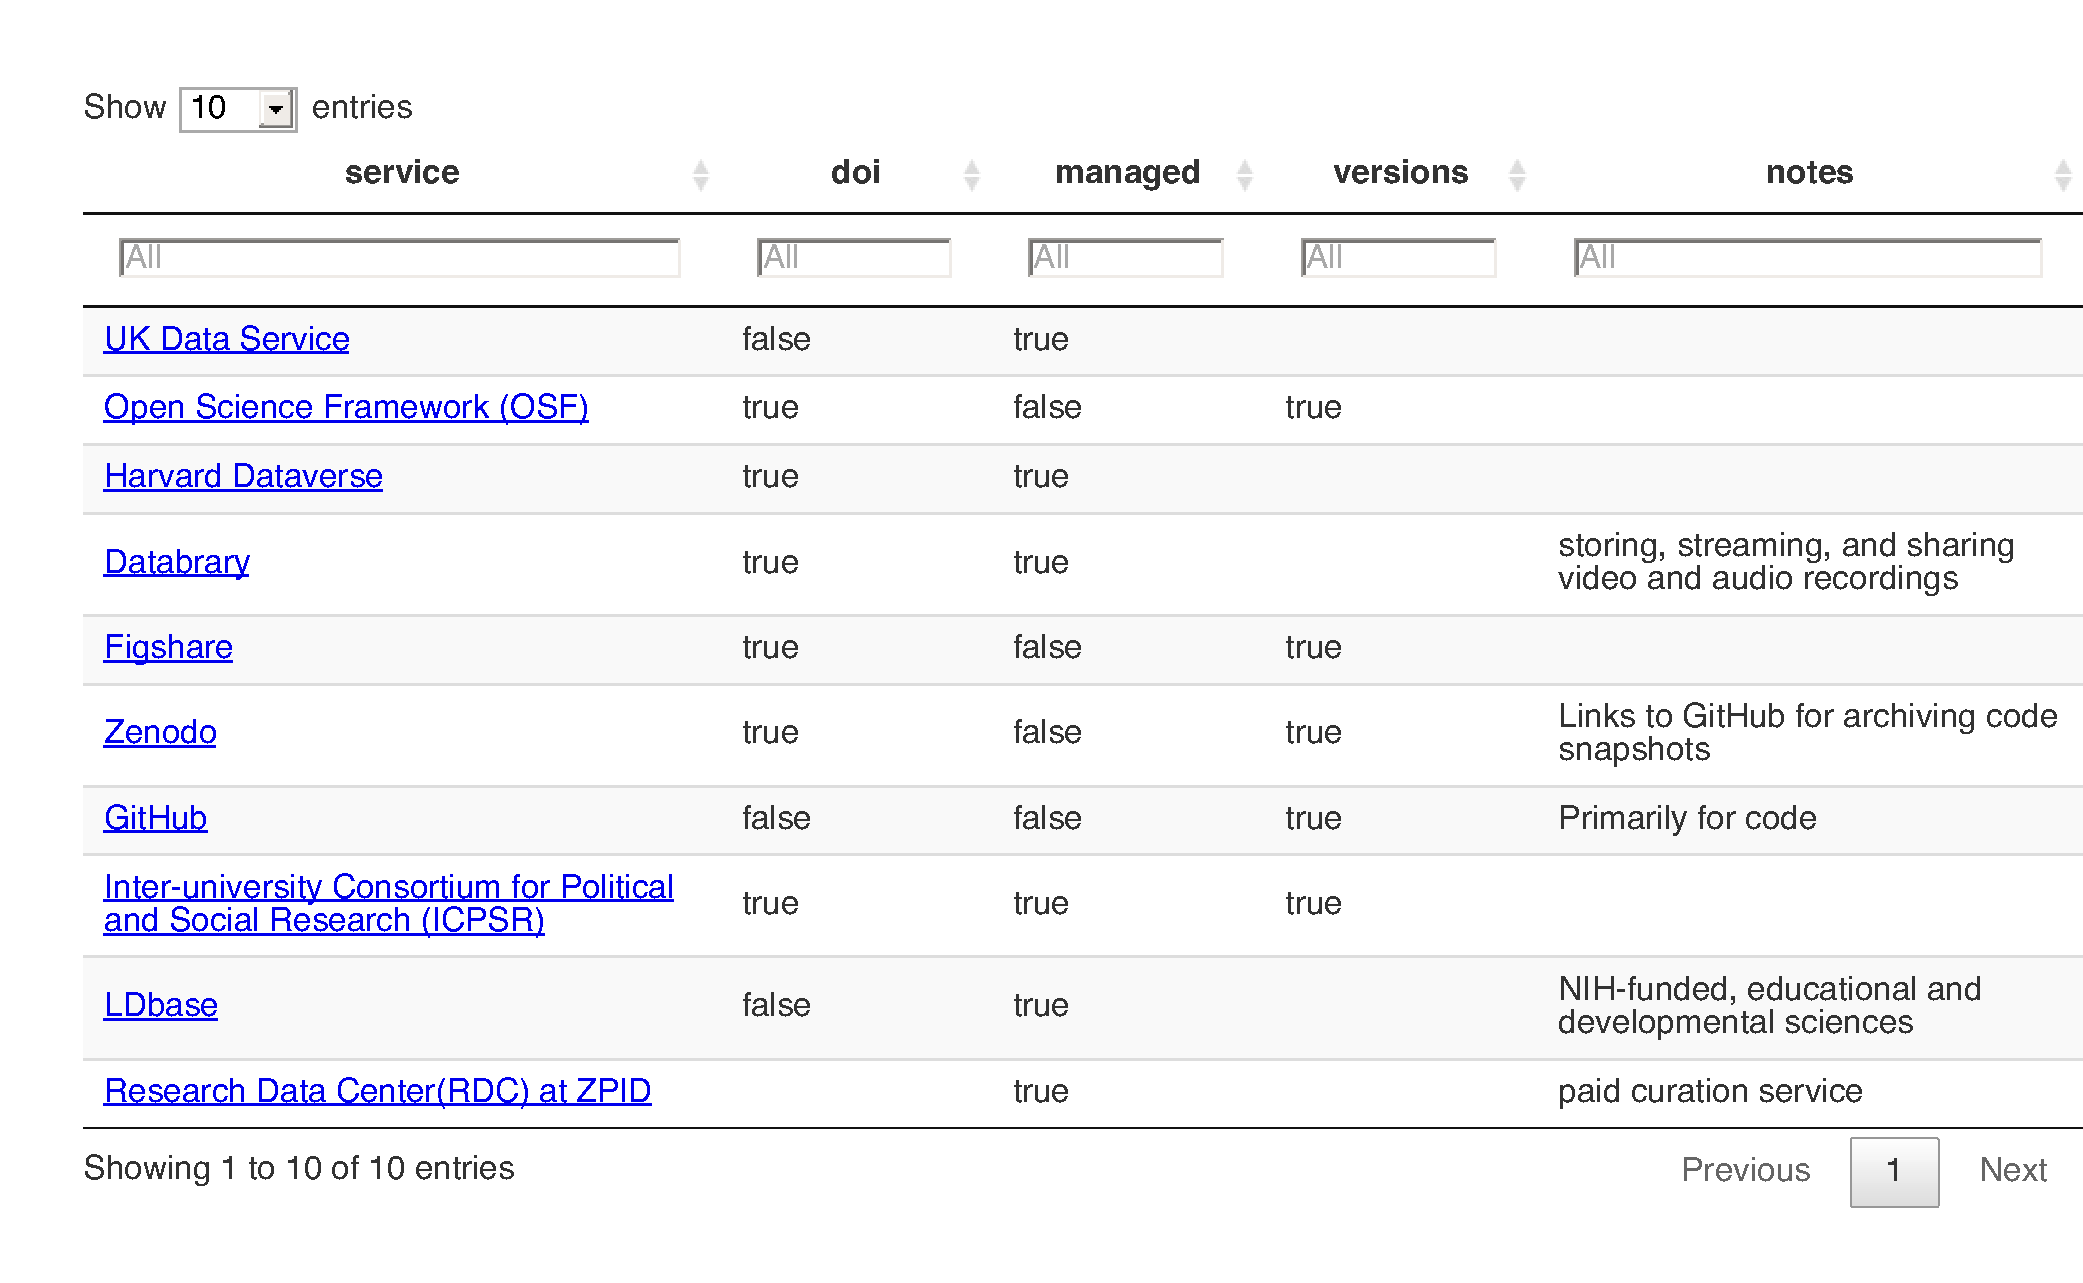
\includegraphics[width=1\linewidth]{open-guide_files/figure-latex/unnamed-chunk-7-1} \end{center}

\hypertarget{registries}{%
\section{Registries}\label{registries}}

\href{https://osf.io/preprints/metaarxiv/zry2u}{Comparison of Preregistration Platforms} \citep{haroz_2022}

\begin{figure}

{\centering 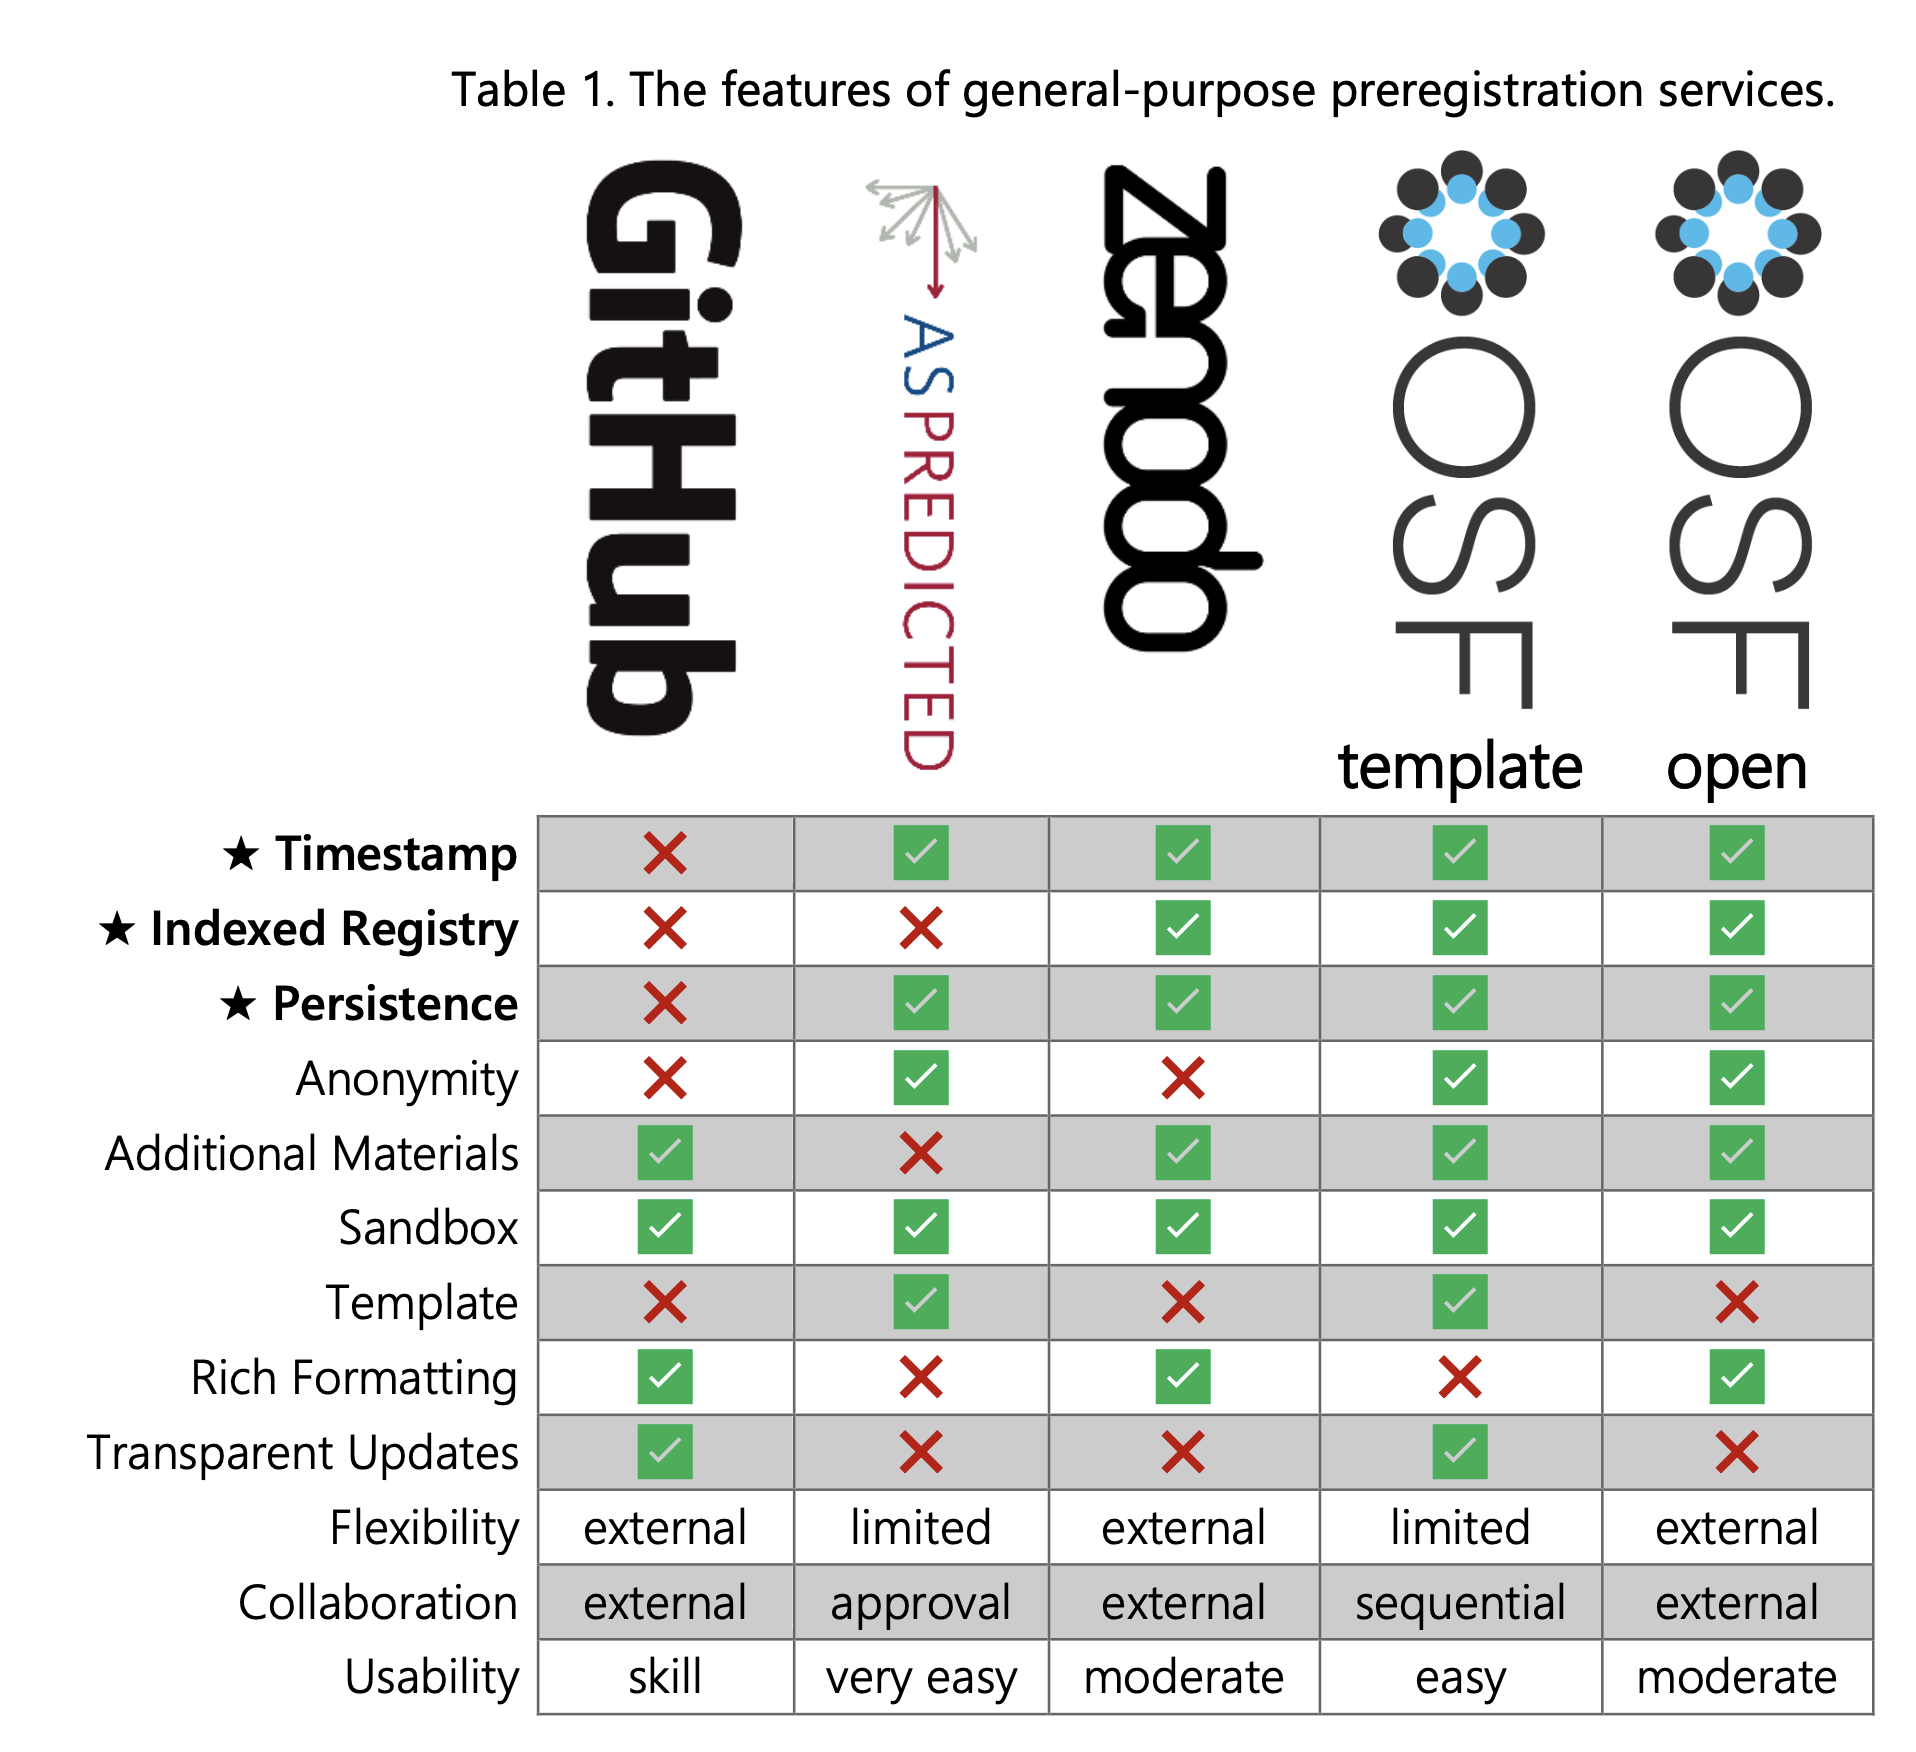
\includegraphics[width=1\linewidth]{images/reg-repos-haroz} 

}

\caption{Figure reproduced from Haroz, 2022}\label{fig:unnamed-chunk-8}
\end{figure}

\begin{itemize}
\tightlist
\item
  \href{https://aspredicted.org/}{As Predicted}
\item
  \href{https://clinicaltrials.gov/}{ClinicalTrials.gov}
\item
  \href{https://osf.io}{Open Science Framework (OSF)}
\item
  \href{https://www.socialscienceregistry.org/}{The American Economic Association's registry for randomized controlled trials}
\item
  \href{https://egap.org/registry-0/}{EGAP Design Registration}
\item
  \href{http://ridie.3ieimpact.org/}{Registry for International Development Impact Evaluations}
\item
  \href{https://osf.io/rr/}{OSF Registered Report protocol registration}
\end{itemize}

  \bibliography{bib.bib}

\end{document}
